\documentclass[journal]{IEEEtran}
\usepackage{cite}
\usepackage{comment}
\usepackage[cmex10]{amsmath}
\usepackage[pdftex]{graphicx}
\usepackage{booktabs} % for toprule
\usepackage{cite, array, times ,fontenc , url, epstopdf, xcolor, tabularx, soul}
\newcommand\todo[1]{\textcolor{red}{#1}}
\newcommand\marc[1]{\textbf{\color{red} /* #1 (marc) */}}
\newcommand\tom[1]{\textbf{\color{orange} /* #1 (tom) */}}
\sethlcolor{white}
\usepackage[algo2e, noend, noline, linesnumbered]{algorithm2e}
\DontPrintSemicolon
\makeatletter
\newcommand{\pushline}{\Indp}% Indent
\newcommand{\popline}{\Indm}
\makeatother


%%
\graphicspath{{img/}}
\DeclareGraphicsExtensions{.pdf,.jpg,.png,.eps}

\begin{document}
\title{Real-time Monte-Carlo Tree Search in Ms~Pac-Man}
\author{Tom~Pepels, Mark~H.M.~Winands, and Marc~Lanctot%
\thanks{Tom Pepels is a student member of the Games and AI Group, Department of Knowledge Engineering, Faculty of Humanities. Email: {\tt tom.pepels@maastrichtuniversity.nl}; 
Mark Winands and Marc Lanctot are members of the Games and AI Group, Department of Knowledge Engineering, Faculty of Humanities
and Sciences, Maastricht University, Maastricht, The Netherlands. 
Email: {\tt \{m.winands, marc.lanctot\}@maastrichtuniversity.nl}
}}
% The article headers
\markboth{Transactions on Computational Intelligence and AI in Games,~Vol.~?, No.~?, Submitted April~2013}%
{On Real-time Monte-Carlo Tree Search in Ms~Pac-Man}
\maketitle

\begin{abstract}
%\boldmath
In this article, Monte-Carlo Tree Search (MCTS) is introduced for controlling the Pac-Man character in the real-time game Ms~Pac-Man. MCTS is used to find an optimal path for an agent at each turn, determining the move to make based on the results of numerous randomized simulations. Several enhancements are introduced in order to adapt MCTS to the real-time domain. Ms~Pac-Man is an arcade game, in which the protagonist has several goals but no conclusive terminal state. Unlike games such as Chess or Go there is no state in which the player wins the game. Instead, the game has two subgoals, 1) surviving and 2) scoring as many points as possible. Decisions must be made in a strict time-constraint of 40 ms. The Pac-Man agent has to compete with a range of different ghost teams, hence limited assumptions can be made about their behavior. In order to expand the capabilities of existing MCTS agents, four enhancements are discussed: 1) a variable-depth tree, 2) simulation strategies for the ghost team and Pac-Man, 3) including long-term goals in scoring, and 4) re-using the search tree several moves with a decay factor $\gamma$. The agent described in this article was entered in both the WCCI'12 and the CIG'12 Pac-Man vs Ghost Team competition, where it achieved a second and first place, respectively. In the experiments we show that using MCTS is a viable technique for the Pac-Man agent. Moreover, the enhancements improve overall performance against four different ghost teams.
\end{abstract}
\begin{IEEEkeywords}
Pac-Man, MCTS, Monte-Carlo, Real-time
\end{IEEEkeywords}
\IEEEpeerreviewmaketitle

\section{Introduction}
\IEEEPARstart{M}{s Pac-Man} is a real-time arcade game based on the popular Pac-Man game released in 1980. The player controls the main character named Ms~Pac-Man (henceforth named \emph{Pac-Man}) through a maze, eating pills and avoiding or chasing the four hostile ghosts. This article discusses enhancements to the Monte-Carlo Tree Search (MCTS) \cite{kocsis2006bandit, coulom2007efficient} framework to allow its use in real-time, stochastic domains such as Ms Pac-Man. 

MCTS has been successful when applied to several types of domains such as puzzles, card games, and board games \cite{brownesurvey}. However, research on real-time domains has been limited in comparison. MCTS has been applied to tactical assault planning in real-time strategy games~\cite{balla2009uct}, steering in the Physical Traveling Salesman Problem~\cite{powleytsp}, and real-time hospital patient admissions planning~\cite{zhu13realtime}. These domains have unique characteristics that make planning more challenging than in the standard turn-based games. For example, computation time for search is often severely limited, the action spaces are large if not infinite, the state spaces are often continuous, and payoffs are sometimes not classified as either wins or losses. 

In Ms Pac-Man, the player's goal is to avoid being eaten by the ghosts and gaining higher scores by collecting pills. Ms~Pac-Man inherited its game-mechanics from the original Pac-Man. Moreover, it introduced four different mazes, and more importantly, unpredictable ghost behavior. Ms~Pac-Man has become an interesting subject for AI research. The game rules are straightforward, however complex planning and foresight are required for a player to achieve high scores. Additionally, the organization of recurring competitions provides a testbed to compare performance between different methods.

In 2007 the first Ms~Pac-Man competition was organized, the \emph{Ms~Pac-Man Competition (screen-capture version)} \cite{mspacmanscreencap}. In this competition Pac-Man agents play the original version of the game in an emulator. Agents interpret a capture of the screen to determine the game state, at each turn moves are passed to the emulator running the game. Games are played by a single Pac-Man agent, competing to get the highest average score over a number of games. Whereas the ghosts behave according to a fixed, known strategy.

In 2011 a second competition was introduced, the \emph{Ms~Pac-Man vs Ghosts Competition} \cite{mspacmanvsghost}. This competition is played in a newly developed implementation of the game, in which the game state is fully available. Furthermore, Pac-Man agents compete with a variety of ghost teams also entered in the competition. The Pac-Man agents compete to get the highest scores, whereas the ghost teams compete for the lowest Pac-Man scores.

Although most Pac-Man agents entering these competitions are rule-based, research has been performed on using general techniques, such as genetic programming \cite{alhejali2010evolving}, neural networks \cite{lucas2005evolving}, and search trees \cite{robles2009simple}. Due to the successful application of MCTS in other games \cite{brownesurvey}, interest in developing MCTS agents for Ms~Pac-Man has grown. Samothrakis \emph{et al.} \cite{samothrakis2011fast} developed an MCTS agent using a Max$^{n}$ search tree with score-keeping for both Pac-Man and the four ghosts separately. Their method sets a target location in the current maze as a long-term goal for Pac-Man while MCTS computes the optimal route to the target in order to determine the best move. Other Monte-Carlo based agents were developed for achieving specific goals in Ms Pac-Man, such as ghost avoidance \cite{tong2010monteghost} and endgame situations \cite{tong2011monteendgame}, demonstrating the potential of Monte-Carlo methods for Pac-Man agents. 
In 2011, the first MCTS agent won the Ms~Pac-Man screen-capture competition \cite{mspacmanscreencap}. Until then, rule-based agents lead the competition. The victorious MCTS agent, {\sc Nozomu} \cite{ikehata2011monte}, was designed to avoid so-called `pincer moves', in which every escape path for Pac-Man is blocked. The approach was successful in beating the leading rule-based agent {\sc ICE Pambush} \cite{thawonmas2010evolution} with a high score of 36,280. In the same year, the first MCTS-based agents entered the Ms~Pac-Man vs Ghosts Competition. Both a ghost team \cite{iceguct, iceguctcig11} and a Pac-Man agent \cite{icepambushcig11} based on a combination of knowledge rules and MCTS search entered the competition. Moreover, the MCTS-based ghost team {\sc nqkien} \cite{iceguct, nguyen2011applying, nguyenmonte} won the CEC'11 \cite{cec11rankings} edition of the competition with an average of 11,407 points scored by its opponents. 

 This article discusses the Pac-Man agent {\sc maastricht}, which won the CIG'12 Ms~Pac-Man vs Ghosts Competition. The agent has full access to the game state and competes with a range of different ghost teams. The goal of this research is to develop a generally strong playing Pac-Man agent based on MCTS. To employ the MCTS framework for Pac-Man four enhancements are introduced: 1) a variable-depth tree, 2) simulation strategies for the ghost team and Pac-Man, 3) including long-term goals in scoring, and 4) re-using the search tree over several moves.
This article is an extension to the CIG'12 conference paper \cite{enhancementspacmancig12} published in 2012. Foremost it focuses on dealing with the real-time aspects of the game. We introduce a strategy to reuse the search tree in order to increase the number of simulations on which to base decisions. Moreover, enhancements to the simulation strategy and long-term goals are detailed, and more extensive experiments are performed against different ghost teams.

The article is structured as follows. First, the Ms~Pac-Man domain is introduced. Next, MCTS and the UCT selection policy are described, and enhancements to the MCTS framework discussed in detail. Finally, experimental and competition results are presented and a conclusion drawn.

\section{Ms Pac-Man}
\label{rules}
The rules of Ms~Pac-Man are based on the classic arcade game. Pac-Man initially has three lives, which she loses through contact with a non-edible ghost. After losing a life due to being captured by a ghost, the location of all the ghosts and Pac-Man are reset to their initial configuration. The game environment consists of four different mazes, which are cycled alternately through the levels. The game progresses every \emph{time unit} of 40 ms., forcing Pac-Man to make a move, i.e. up, down, left, or right. Pac-Man cannot explicitly skip a turn, it is however possible to ``wait'' by moving onto a wall, or reversing the previous move every turn. Ghosts are only allowed to make a move at a junction in the maze. On a path between junctions they can only travel forward. When a power pill is eaten by Pac-Man the ghosts become edible for a limited time: their movement speed decreases and they are instantly forced to reverse their direction. At the moment Pac-Man reaches a score of $10,000$ by eating pills and ghosts, she gains a life. 

Both the ghost team and Pac-Man have one in-game time unit to compute a move. Once computed and submitted, the ghost team's and Pac-Man's moves are executed simultaneously. If no move is submitted, a randomly selected one is executed. Furthermore, at each turn a `global reverse' can occur with a small probability of $0.0015$ where each ghost is immediately forced to reverse its direction. Pac-Man gains $10$ points for each pill eaten, $50$ per power pill, and $200^n$ for each ghost eaten, where $n\in \{ 1, 2 , 3, 4 \}$ is the total number ghosts eaten after taking the power pill. The game either ends naturally when Pac-Man has no lives remaining or after a set time limit.

The version of the game used in the Ms~Pac-Man vs Ghosts competition is two-player, fully observable, asymmetric, and stochastic. This is in contrast with the original version of the game, which was single-player, because the ghosts followed a pre-determined strategy. Specifically, several rules were introduced in the competition to balance its results. The most important rules specific to the CIG'12 version of the competition are, 1) each maze is played for $4,000$ time units, after which the game progresses to the next level, 2) the game ends after a total of $24,000$ time units, and 3) for each life remaining at the end of the game, Pac-Man is rewarded $800$ points. 

\begin{figure}[ht]
	\centering
	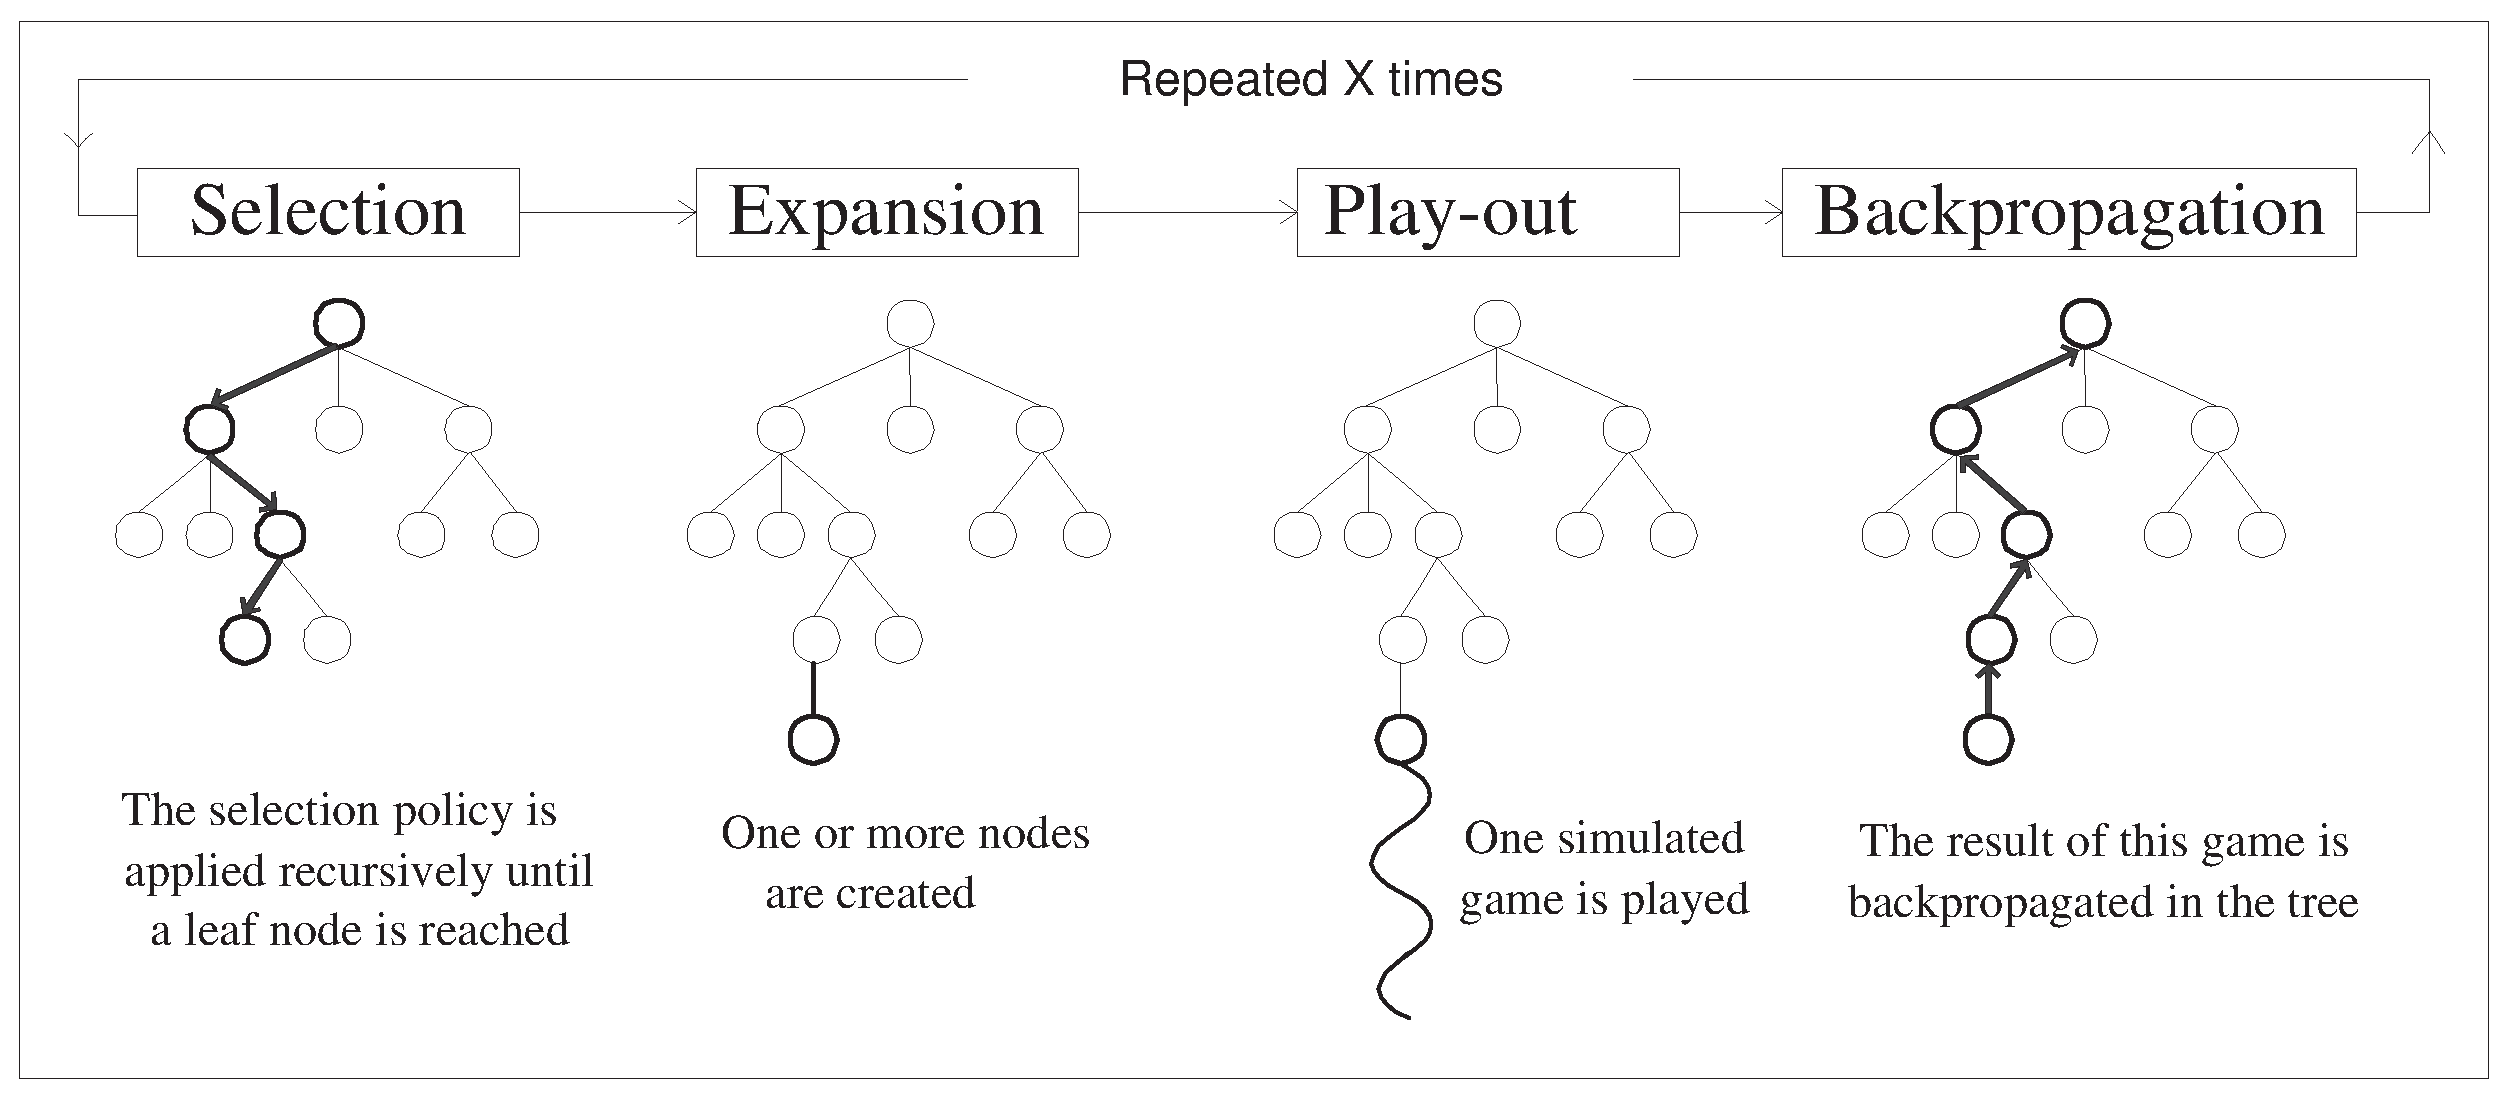
\includegraphics[width=.5\textwidth]{img/figure1.eps}
	\caption{Strategic steps of Monte-Carlo Tree Search \cite{chaslot2008progressive}.}
	\label{fig:mcts-algorithm}
\end{figure}
\section{Monte-Carlo Tree Search}
\label{MCTS}
Monte-Carlo Tree Search (MCTS) is a best-first search method based on random sampling of the state space for a specified domain \cite{kocsis2006bandit},\cite{coulom2007efficient}. In gameplay, this means that decisions are made based on the results of random play-outs. MCTS has been successfully applied to various turn-based games such as Go \cite{lee2010current} and Hex \cite{arneson2010monte}. Moreover, MCTS has been used for agents playing real-time games such as the Physical Traveling Salesman  \cite{powleytsp}, real-time strategy games \cite{balla2009uct}, and Ms~Pac-Man \cite{ikehata2011monte}. A particular challenge for agents playing real-time games is that they are  characterized by uncertainty, a large state space, and open-endedness. However, MCTS copes well when limited time is available between moves as it can be terminated anytime to select a move. Furthermore, the algorithm encapsulates uncertainty in its randomized play-outs \cite{brownesurvey}.

In MCTS, a tree is built incrementally over time and maintains statistics at each node corresponding the rewards collected at those nodes and number of times the nodes have been visited. The root of this tree corresponds to the agent's current position. The basic version of MCTS consists of four steps, which are performed iteratively until a computational threshold is reached, i.e. a set number of iterations, an upper limit on memory usage, or a time constraint. The four steps (depicted in Figure \ref{fig:mcts-algorithm}) at each iteration are \cite{chaslot2008progressive}:
\begin{itemize}
\item {\bf Selection}. Starting at the root node, children are chosen according to a selection policy. When a leaf node is reached that does not represent a terminal state it is selected for expansion.
\item {\bf Expansion}. All children are added to the selected leaf node given available moves.
\item {\bf Play-out}. A simulated play-out is run, starting from the state of the added node. Moves are performed randomly or according to a heuristic strategy until a terminal state is reached.
\item {\bf Backpropagation}. The result of the simulated play-out is propagated immediately from the selected node back up to the root node. Statistics are updated along the tree for each node selected during the selection step and visit counts are increased.
\end{itemize}
The combination of moves selected during the selection and play-out steps form a single \emph{simulation}. During the selection step, moves are executed according to the selection policy, and during play-out moves are performed (semi-)randomly, or according to some simulation strategy.
Because results are immediately backpropagated, MCTS can be terminated anytime to determine the decision to be made. Moreover, no static heuristic evaluation is required. However, in most cases it is beneficial to add domain knowledge for choosing moves made during the play-out. 

\section{Monte-Carlo Tree Search for Ms Pac-Man}
This section discusses the enhancements to the MCTS framework for the Pac-Man agent. The agent builds upon the ideas proposed by Ikehata and Ito \cite{ikehata2011monte}. First, a description of the search tree is provided. In subsequent sections, the reward structure and individual enhancements to the strategic steps of MCTS are given. The goal is to present techniques that are both specific to Ms~Pac-Man, but could also be extended or adapted to other (real-time) domains.

\subsection{Search Tree and Variable Depth \label{sec:stavd}}
The game's environment consists of four different mazes. These can be directly represented as a graph where the \emph{junctions} are \emph{nodes}, and \emph{corridors} between junctions are \emph{edges}. Pac-Man has the option to make a decision at any location in the graph. At a node she has a choice between more than two available directions, while on an edge she can choose to maintain her course or reverse. An example of such a graph is depicted in Figure \ref{fig:maze-gametree}. The associated search tree is shown in Figure \ref{fig:tree}.
\begin{figure}[hb]
	\centering
	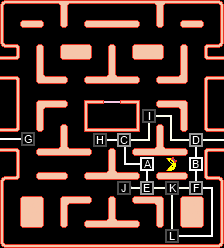
\includegraphics[width=0.26\textwidth]{figure2.png}
	\caption{Graph representation of a game state. All nodes refer to decisions for Pac-Man.}
	\label{fig:maze-gametree}
\end{figure}
\begin{figure}[ht]
	\centering
	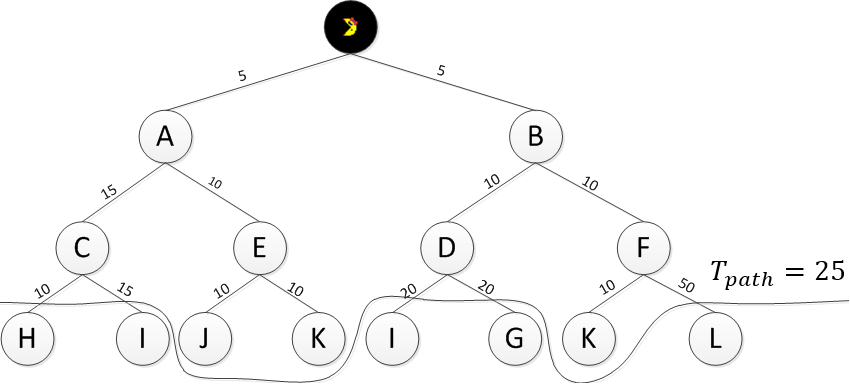
\includegraphics[width=0.4\textwidth]{figure3.png}
\vspace{-4pt}
	\caption{Example tree with a distance limit of 25. Based on the game state in Figure \ref{fig:maze-gametree}.}
	\label{fig:tree}
\vspace{-4pt}
\end{figure}

Decisions in the tree are the moves made at nodes, i.e. junctions in the maze. Traversing the tree during the selection step means that Pac-Man moves along an edge until a node is reached. At this point either a leaf is reached and play-out starts, or a new edge is chosen based on a child of the current node. The tree represents a distinct discretization of Ms~Pac-Man's complex overall game state. As the tree is \emph{single-player}, the movements of the ghosts are not represented by nodes \cite{ikehata2011monte}. Instead, they are simulated based on a simulation strategy, while Pac-Man traverses the tree. As such, even within the tree, game states are approximations. Contrasting the approach used in traditional games, where both the player and opponent(s) have decision nodes in the tree, and the game state represented by a node models the game state exactly for both players.

Within the tree, \emph{reverse moves}, i.e. moves that lead back to a parent, are not considered beyond the first ply. When a node $n_p$ representing junction $j_p$ is expanded, each child $n_i$ represents a move that leads to a different junction $j_i$ in the maze, excluding junction $j_p$. Reverse moves are not considered deeper in the tree to ensure a larger difference in rewards between available moves. If reverse moves are expanded on every ply, more simulations per move are required in order to have conclusive differences in rewards. Considering, 1) in total, more nodes are expanded, and 2) the tree contains duplicate paths with similar or equal rewards.

Each node stores three different reward values, $tactic \in \{ghost, pill, survival\}$, both cumulative and maximized over their children's values. Suppose that node $p$, with a set of children $C(p)$ has been visited $N$ times. Furthermore, simulations made through $p$ resulted in rewards $R_{tactic, n}^p$ where $n\in\{1,2, \dots, N\}$. The cumulative sum of rewards stored at $p$ is:
\begin{equation}
S_{tactic}^p = \sum_{n = 1}^{N}{R_{tactic,n}^p} 
\end{equation}
where the rewards of simulation $n$ through node $p$, i.e. $R_{ghost, n}^p$, $R_{pill, n}^p$ and $R_{survival, n}^p$, respectively, 
are defined in more detail in Subsection \ref{simulation}. 
The mean reward is then defined as 
\[\bar{S}_{tactic}^p = \frac{S_{tactic}^p}{N}.\]
The maximum mean reward is defined recursively as
\begin{equation}
M_{tactic}^p =
\begin{cases}
   \bar{S}_{tactic}^p & \text{if $p$ is a leaf}, \\
   -\infty & \text{if $p$ is not in the tree}, \\
   \max_{i \in C(p)}{M_{tactic}^i} & \text{otherwise}.
\end{cases}
\label{eq:maxback}
\end{equation}

Reward quantities $M_{tactic}$ and $\bar{S}_{tactic}$ are both in $[0,1]$. $M_{tactic}$ is used when determining the value $v_i$ for each move during selection, backpropagation, and deciding the move to make based on the current tactic. The different tactics are discussed in the next subsection.

Ikehata and Ito \cite{ikehata2011monte} used a search tree restricted in depth to a fixed number of edges, without regard for the distance these edges represent in-game. Although the search tree in this article is constructed similarly, the search path is variably determined by a distance limit $T_{path}$. A leaf is only expanded if the length of the path to the root node does not exceed $T_{path}$ (as shown in Figure \ref{fig:tree}). In Ms~Pac-Man, distance units are represented using some internal measure, i.e. the distance between two consecutive pills is $4$. The variable-depth search prevents the agent from choosing `quick fixes' when in danger, i.e. it may be safer to traverse a short path in the game when Pac-Man is in danger, than a long path which could be the case when tree-depth is limited by a fixed number of edges. Furthermore, the scoring potential over all possible paths in the tree is normalized due to the uniform length of each path.

\subsection{Tactics}
\label{Strategy}
According to the current game state, a tactic \cite{ikehata2011monte} for determining the behavior of Pac-Man is selected. Tactics are based on the three subgoals of Pac-Man, and is dependent on the safety of the current position. Which tactic to choose is determined by setting a constant threshold $T_{survival}$, based on the highest survival rate of current simulations. At any time, one of the following is active \cite{ikehata2011monte}:
\begin{itemize}
\item The {\bf Ghost score} tactic is selected if a power pill was eaten in a previous turn, edible ghosts are in the range of Pac-Man, and the maximum survival rate is above the threshold $T_{survival}$.
\item The {\bf Pill score} tactic is the default tactic. It is applied when there are no edible ghosts in range, and the maximum survival rate is above the threshold $T_{survival}$.
\item The {\bf Survival} tactic is used when the maximum survival rate of the previous or current search is below the threshold, $T_{survival}$.
\end{itemize}

Survival heuristics have been used previously in sudden-death games such as Connect6 \cite{yen2011two}. However, unlike previous work, here we consider the different tactics for the purposes of rewards. Moreover, the current tactic is determined before MCTS starts and reassessed at every search. 

The $v_i$ value used for selection, backpropagation, and the final move selection is based on the current tactic. It is either the maximum survival rate when the survival tactic is active, or the current score multiplied by the survival rate for the ghost and pill tactics, respectively.
$v_i$ is defined as follows:

\begin{equation}
v_i =
\begin{cases}
   {M}^i_{ghost} \times {M}^i_{survival} & \text{if $tactic$ is $ghost$}, \\
   {M}^i_{pill} \times {M}^i_{survival} & \text{if $tactic$ is $pill$}, \\
   {M}^i_{survival} & \text{if $tactic$ is $survival$}.
\end{cases}
\label{eq:vi}
\end{equation}

For the $ghost$ and $pill$ tactics the maximum survival rate ${M}^i_{survival}$ is used as a predictive indicator that the node's reward will be achieved in the long term.

% Perhaps we should place the subsection on backpropagation here

\subsection{Search Tree Reuse}
\label{reuse}
In real-time environments where fast decision making is required, MCTS may be at a disadvantage compared to strong rule-based algorithms. The quality of Monte-Carlo sampling methods depend on the number of samples, i.e. more samples lead to better approximations, which allows for stronger play. However, the real-time 40 ms. time frame in Ms~Pac-Man severely limits the number of simulations possible. 

In Ms Pac-Man, long-term reasoning is done using a preference relation over goals. That is, when Pac-Man makes a plan $P_k$ to follow a path, out of the possible plans $P_{1 \ldots i}$, there exists a preference relation at the current turn such that $P_k \succ \{P_1, \ldots, P_i\} \backslash P_k$. In subsequent turns, Pac-Man either confirms or denies the relevance of the current preference. Reasons to deny it in a later turn could be that Pac-Man would be in danger if she kept following the current plan, or there is an opportunity to score many points on an alternative path. However, if such a reason does not exist the preference should be maintained until it no longer holds.

Rebuilding a new search tree at each turn restricts long-term planning. Since the information collected at each previous search is lost, the agent can become fickle and constantly switch back and forth between high-level preferences. However, reusing the search tree and its values each turn without modification can lead the agent to become too stubborn. Values collected from previous turns may become outdated, and consequently many new results may be required to overcome biases formed from past searches. 

We combine two techniques for reusing the search tree between successive searches. The first technique uses a rule-base to determine when the game state has significantly changed indicating that the values stored in the tree are no longer relevant. The second technique decays the values stored in the tree between successive turns. This decay ensures that sample results from previous turns still play a role in making new decisions, but the importance of past results lowers over time. This decay is important because values collected in the past were based on a situation that may have changed. However, in real-time domains, the state changes between successive turns are often small and so the information collected in previous searches often remains relevant.  

{\sc rule-based reuse.} When reusing the search tree and its values, the game state can change in a manner not predicted by the search. In this case, values from previous searches should be discarded to make place for a new tree that represents the current game state. These cases were identified and constructed into a rule base. If any of the following is true, the existing tree is discarded, and a new tree is built:
\begin{itemize}
\item Pac-Man has died, or entered a new maze.
\item Pac-Man ate a blue ghost or a power pill. This ensures that the search can immediately focus on eating (the remaining) ghosts.
\item There was a global reverse. If all ghosts are forced to reverse, values of the previously built search tree certainly no longer reflect the game state.
\end{itemize}

{\sc continuous decay.} Values stored at nodes can be discounted to decay them over time, implying the continuous use of results throughout consecutive moves. The decay is achieved by multiplying each node's cumulative scores, $S_{ghost}$, $S_{pill}$, and $S_{survival}$, and visit count by $\gamma$ at the start of each turn. Next, the search is performed with each node in the tree initialized with these discounted values. During the selection step and final move selection, the value of a node is determined by combining the decayed values, and the rewards of simulations made during the current move.

Re-using the tree implies that at the start of each move either a new root is selected based on Pac-Man's last move, or a new tree is built. If Pac-Man's last location was a junction, the new root is the first-ply child that corresponds to the last move selected. Next, the tree is restructured to make sure no reverse moves exist beyond the first ply. Moreover, the lengths of the paths in the tree are updated such that they correspond to the actual distances in the game. Lastly, the values stored at nodes that were altered are updated such that they equal the sum of their children.

The decaying of information we propose differs from previous applications of discounting used in MCTS. Discounted UCB was described on the multi-armed bandit problem in \cite{Kocsis06ducb} and \cite{Garivier11On}. Discounted UCT is the application of Discounted UCB to the tree case. In Discounted UCT, discounting is applied every time a node is visited during the search. The rationale in this scheme is that earlier searches are biased by less informed choices since subtrees below each move have not been sufficiently explored, and so discounting is proposed to remove some of this bias. Discounting in this way did not appear to improve performance in Othello, Havannah, and  Go~\cite{Hashimoto12Accelerated}. When using a different MCTS algorithm (BRUE), this form of discounting has been shown to work better in practice in some domains and leads to a different bound on simple regret~\cite{Feldman12Simple}. Accelerated UCT also discounts the node's values during the search but does so non-uniformly by taking into account each move's relative visit frequency~\cite{Hashimoto12Accelerated}. 

In our case, a single discount is applied to all nodes in the tree between successive searches. The idea is to gradually decrease the importance of rewards collected over {\it states further from the root} similar to how future rewards are discounted in Markov Decision Processes~\cite{Bertsekas12MDPbook} and reinforcement learning~\cite{sutton1998reinforcement}. This form of discounting during tree reuse may be appropriate in Ms Pac-Man since the brief search time leads to less accurate approximations, and the nodes in the tree do not perfectly model the actual state in the game due to abstraction assumptions. Searches performed later will in any case have a more up-to-date, and therefore more accurate, model of the actual game state.

Previous work used discount factors to decay heuristic values maintained to guide simulation strategies~\cite{tak13decaying}. The results suggest that decaying these values ($0 < \gamma < 1$) can help in the simulation strategies compared to no decay ($\gamma = 1$) and no reuse ($\gamma = 0$).

\subsection{Selection and Expansion}
\label{uct}
During the selection step, a policy is required to explore the tree for rewarding decisions and finally converge to the most rewarding one. The Upper Confidence Bound applied to Trees (UCT) \cite{kocsis2006bandit} is derived from the UCB1 policy \cite{auer2002using} for maximizing the rewards of a multi-armed bandit. UCT balances the exploitation of rewarding nodes whilst allowing exploration of lesser visited nodes. The policy that determines which child to select given the current node is the one that maximizes the following equation:
\begin{equation}
\label{eq:uct}
X_i = v_i + C \sqrt{ \frac{\ln{n_p}}{n_i}}
\end{equation}
$v_i$ is the score of the current child based on the active tactic, defined in Equation \ref{eq:vi}. In the second term, $n_p$ is the visit count of the node and $n_i$ the visit count of the current child. $C$ is the exploration constant to be determined by experimentation.

The UCT selection policy is used when the visit count of all children are above a threshold $T$ \cite{coulom2007efficient}. When one or more of the children's visit counts are below this threshold, a random uniform selection is made. In the case of Ms~Pac-Man, the threshold used is 15, which ensures a high confidence on the safety of the path. An otherwise safe and/or rewarding node may have resulted in a loss the first time it is expanded, due to the stochastic nature of the game. Using the threshold ensures that this node is explored again, increasing the confidence on the safety and reward of the decision.

\subsection{Simulation}
\label{simulation}
During simulation (the combined selection and play-out steps), Pac-Man and the ghosts simultaneously make moves in a fully functional game state. Pac-Man's moves are determined by either the fixed selection performed by UCT, or a simulation strategy described in the next subsection. Therefore, simulation consists of two parts: 1) the \emph{selection step}, and 2) the \emph{play-out step}. Ghosts move according to their simulation strategy during both these steps, and have no fixed strategy determined by selection.

During the selection step, moves corresponding to each visited node during selection (Subsection \ref{uct}) are performed by Pac-Man. This provides the basis for determining the achievable score of a path in the tree, while allowing for Pac-Man to be captured by the simulated ghost team. Whenever selection ends or is interrupted, play-out begins and both Pac-Man and the ghosts move according to the simulation strategy.

There exist two cases in which the selection step can be interrupted due to an unpredictable change in the game state:
\begin{enumerate}
\item If Pac-Man loses a life during the selection step, a play-out is started from the last-visited junction. Losing a life during the selection step is basically a suicide move, as Pac-Man may only travel forward without regard for safety. Therefore the play-out is run starting from the last junction, to determine whether Pac-Man could have avoided the loss of life. 
\item Pac-Man eats a ghost or a power pill, in this case play-out is started immediately. However, if there are edible ghosts active and a power pill is eaten, simulation terminates immediately. This prevents Pac-Man from ``wasting'' power pills.
\end{enumerate}
In both cases, the result of the simulation is backpropagated from the last visited junction, i.e. node in the search tree. Note that, in this case it is not the leaf visited during selection that gets updated, rather backpropagation is started at an internal node. However, if the selection step is not interrupted, play-out starts from the junction represented by the leaf.

A game of Ms~Pac-Man ends when either Pac-Man loses all lives, or after $24,000$ time units. It is neither useful nor computationally achievable within the strict time limit of 40 ms. to run numerous simulations until one of these conditions holds. Running long play-outs introduces bias for MCTS in favor of the heuristics used. Moreover, it updates the tree with results based on long-term estimations on the game state, which are neither accurate nor interesting for evaluating the current state.

The goal of the play-outs is to determine the short and long-term safety and reward of a selected path. Therefore, different \emph{stopping conditions} should be used. Two natural stopping conditions can be considered, either Pac-Man loses a life (dies), or the game progresses to the next maze. However, to prevent lengthy play-outs, additional stopping conditions are introduced. Therefore, during play-out, moves are made until one of the following four conditions applies:
\begin{enumerate}
\item A pre-set number of time units $T_{time}$ have passed \cite{ikehata2011monte}.
\item Pac-Man is considered dead, i.e.:
\begin{itemize}
\item Came into contact with a non-edible ghost.
\item Is trapped at the end of the play-out, every available path is blocked by ghosts.
\end{itemize}
\item The next maze is reached.
\end{enumerate}
$T_{time}$ is determined by adding the distance limit of the search tree, $T_{path}$ with a simulation time-constraint $T_{simulation}$. This ensures that each simulation has the same length in time and, in effect, the same scoring potential.

When a simulation ends for any of the aforementioned reasons, Pac-Man's score is determined based on the three subgoals of the game. Results of a simulation consist of three values \cite{ikehata2011monte}:
\begin{enumerate}
\item $R_{survival} =
 \begin{cases}
    0 & \text{if Pac-Man died}\\
    1 & \text{if Pac-Man survived}
  \end{cases}$
\item $R_{pill} \in [0, 1] $ the number of pills eaten, normalized by the number of pills at the start of the level.
\item $R_{ghost} \in [0, 1] $ the number of ghosts eaten, normalized by the total edible time at the start of the simulation.
\end{enumerate}
These rewards are defined as described in Subsection \ref{longterm}. Each node stores a tuple containing the sum of these individual rewards $S_{ghost}, S_{pill},$ and $S_{survival}$ as defined in Subsection \ref{reuse}.

The goal for Pac-Man during the play-out is acquiring the highest score possible whilst avoiding a loss of life. The ghosts have three goals: 1) ensure that Pac-Man loses a life by trapping her, i.e. every possible path leads to a non-edible ghost, 2) ensure the lowest ghost-reward $R_{ghost}$, which increases when Pac-Man eats edible ghosts, and 3) limit as much as possible the number of pills Pac-Man can eat. To achieve these goals we introduce a simulation strategy for Pac-Man and the ghosts in the next subsection.
\begin{figure}[ht]
	\centering
	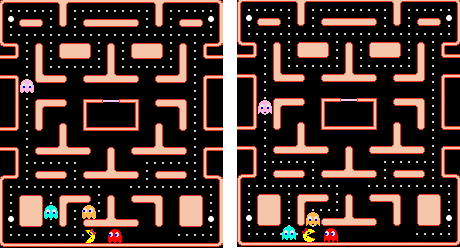
\includegraphics[width=0.45\textwidth]{figure4.png}
	\caption{Ghosts executing a pincer move.}
	\label{fig:pincer}
\end{figure}

\subsection{Simulation Strategy}
\label{simstrat}
During simulation, Pac-Man and the ghost team's moves are executed simultaneously in a fully functional game state, using the complete rule set of the game (Section \ref{rules}). In this subsection the simulation strategies for the ghosts and Pac-Man are detailed. The strategies were designed to ensure that any time Pac-Man does not survive the play-out (Subsection \ref{simulation}), it is due to all possible paths being blocked by ghosts. Therefore, $\bar{S}_{survival}$ can be considered as an indicator of the probability of a \emph{pincer move} occurring along the path.

{\sc ghost simulation strategy}.
The goal of the ghosts is to trap Pac-Man in such a way that every possible move leads to a path blocked by a ghost, i.e. a pincer move (Figure \ref{fig:pincer}). The ghosts therefore are assigned a random target-location vector $\vec{target}$ that determines whether an individual ghost is to approach the front or rear of Pac-Man. This approach is similar to \cite{ikehata2011monte}, with the addition of using a randomized target vector.

Ghosts move based on an $\epsilon$-greedy strategy \cite{sutton1998reinforcement, sturtevant2008analysis}. With a probability $\epsilon = 0.2$ at each turn, a ghost makes a random move. With probability $1-\epsilon$ the ghosts move according to strategic rules, derived from the rules proposed in \cite{ikehata2011monte} and detailed in this subsection.
When selecting a ghost's move during simulation, there are two mutually exclusive cases to consider, non-edible or edible. Moreover, there is a third case, which overrules a selected move in any case.

{\bf Case 1.} If ghost $g_i$ is \emph{not} edible. A move is selected according to the following rules:
\begin{enumerate}
\item The ghost selects a move that immediately traps Pac-Man if available.
\item If the ghost is in the immediate vicinity of Pac-Man, i.e. within $6$ distance units, the ghost moves along the next direction of the shortest path to Pac-Man.
\item If the ghost is closer to the junction that lies in front of Pac-Man than Pac-man is herself, and $\vec{target_i} = front$, then the ghost will move directly to Pac-Man's forward junction, which essentially blocks her forward path.
\item If the ghost is on a junction directly connected to the edge that Pac-Man is located on and if no other ghost is on the edge moving in the same direction, then the ghost chooses the move that leads to this edge, blocking Pac-Man based on the $ \vec{target_i}$ designation.
\item Otherwise, the ghost moves closer to the assigned target location. Based on the value of $\vec{target_i}$, the target is either the nearest junction in front or behind Pac-Man.
\end{enumerate}
\begin{figure}[t]
	\centering
	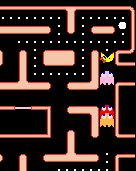
\includegraphics[width=0.2\textwidth]{figure5.png}
	\caption{Ghosts chasing Pac-Man from similar distance and location.}
	\label{fig:badchase}
\end{figure}

{\bf Case 2.} If ghost $g_i$ is edible, a move is chosen that maximizes the distance between him and Pac-Man.

{\bf Case 3.} If a ghost is to move on an edge currently occupied by another ghost moving in the same direction, the move is eliminated from the ghost's selection and a different move is selected randomly. This policy ensures that ghosts are spread out through the maze, increasing their possible trapping or catching locations. It also prevents multiple ghosts from chasing Pac-Man at the same (or similar) distance and location shown in Figure \ref{fig:badchase}.

{\sc pac-man simulation strategy}. Moves made by Pac-Man are prioritized based on safety and possible reward. When more than one move has the highest priority, a move is chosen at random. Before discussing the strategy in detail, the concept of a \emph{safe move} has to be defined first. A safe move is any move that leads to an edge which:
\begin{itemize}
\item has no non-edible ghost on it moving in Pac-Man's direction, and
\item whose next junction is safe, i.e. in any case Pac-Man will reach the next junction before a non-edible ghost.
\end{itemize}

During play-out Pac-Man moves according to the following set of rules. If Pac-Man is at a junction the following rules apply, sorted by priority:
\begin{enumerate}
\item If there are reachable edible ghosts, i.e. the traveling time it takes to reach to a ghost is smaller than its edible time remaining, then select a safe move that follows along the shortest path to the nearest edible ghost.
\item If a safe move leads to an edge that is not cleared, i.e. contains any number of pills, it is performed.
\item If all safe edges are cleared, select a random move leading to a safe edge.
\item If no safe moves are available, a random move is selected \cite{ikehata2011monte}.
\end{enumerate}

If Pac-Man is on an edge, she can either choose to maintain her current course or reverse it. The following rules consider the cases when Pac-Man is allowed to reverse:
\begin{itemize}
\item There is a non-edible ghost heading for Pac-Man on the current path.
\item A power pill was eaten, in this case the move that leads to the closest edible ghost is selected.
\end{itemize}
In any other case Pac-Man continues forward along the current edge. Note that, if Pac-Man previously chose to reverse on the current edge, she may not reverse again until she reaches a junction. Moreover, to improve the performance of play-outs, checking the first condition is only performed if the last move made at a junction was based on an unsafe decision.

\subsection{Long-Term Goals}
\label{longterm}
Time is an important aspect of Ms Pac-Man. Ghosts need to be eaten as fast as possible, and remaining in a maze longer than necessary increases the risk of being captured and decreases the total time available for scoring points. Furthermore, after 10,000 points, Pac-Man gains a life. These are examples of long-term goals in the game. Any MCTS implementation looks at short-term rewards when running simulations. To estimate the rewards of these long-term goals, specific results are considered for both pill and ghost rewards.

To encode the long-term goal in the ghost reward $R_{ghost}$, its immediate reward when eating a ghost is the edible time remaining before the ghost was eaten. This ensures there is a preference for eating ghosts as fast as possible. Furthermore, when Pac-Man eats a power pill (while no edible ghosts are active) during simulation, she must achieve a ghost score higher than 0.5 at the end of the play-out. If this is not the case, i.e. the ghosts were too far away to be eaten in time, the pill-reward $R_{pill}$ is 0. If the minimum ghost score of 0.5 is achieved after eating a power pill, the pill-reward is increased: $R_{pill} = R_{pill} + R_{ghost}$. This rapid change in scores enables Pac-Man to wait for the ghosts to be close enough before eating a power pill.

There are only four power pills available per maze to provide a guaranteed safe escape. In addition, clearing a maze fast increases the scoring potential as the game ends after 24,000 time units. Therefore, eating all pills before the game naturally progresses to the next maze is a beneficial long-term goal. To shape the reward $R_{pill}$ accordingly, we introduce an \emph{edge-reward}. This means that the reward for eating pills is incremented only when an edge is cleared, i.e. the last pill on the edge is eaten. This ensures that Pac-Man prefers to eat all pills on the edges she visits, rather than leaving isolated pills, which become hard to reach as the game progresses. On the one hand, long edges in the maze have a higher scoring potential, on the other hand, they pose a greater risk for Pac-Man. Therefore, it is generally beneficial to clear long edges when it is safe to do so. Although the edge-reward resolves the issue partially, clearing several short edges may still result in a larger reward than clearing a single, long edge. To incorporate this non-linear goal in scoring, the edge-reward is defined as follows: $R_{edge} = {num\_pills(e_i)}^{p}$ where $1 < p < 2$ and $e_i$ represents the edge cleared. This ensures that long edges provide relatively higher rewards while constricting the maximum reward per edge. In this case $R_{pill} = \max(R_{pill}, R_{edge})$ and is normalized based on the total number of pills in the maze. This ensures that the simulation is properly rewarded, even if no edges were fully cleared.


\subsection{Backpropagation and Move selection \label{sec:bpms}}

Results are backpropagated from either the expanded leaf node, or the internal node reached in the interrupted selection step, to the root based on maximum backpropagation \cite{coulom2007efficient}. Scores stored at each internal node represent the maximum scores of its children based on $v_i$ according to the current tactic, as defined in Equation \ref{eq:vi}. Whereas traditionally, MCTS implementations for games use average backpropagation, maximization is applied to MCTS for Ms Pac-Man. During the search when a state is reached, upon return the parent, the maximum score $M_{tactic}$ over the children is returned to the parent. The maximum is used because every move Pac-Man can make at a junction can have altogether different results \cite{ikehata2011monte}. For example, at a given junction Pac-Man has two options to move. A decision to go left leads to a loss of life for Pac-Man in all simulations, whereas a choice to go right is determined to be safe in all simulations. When using average values, the resulting score is 0.5, whereas maximum backpropagation results in the correct evaluation of 1. 

After each simulation, results are incremented starting at the node from which the play-out step was initiated. Next, the values of the parent node are set to the maximum values over all its children. This process is recursively executed until the root is reached according to the definition of $M_{tactic}$ in Equation \ref{eq:maxback}. Children of the root then obtain the scores of their highest-scoring leaf, and the root has the value of the highest scoring node in the tree.

For final move selection, first the current tactic (Subsection \ref{Strategy}) is evaluated. If the maximum survival rate is below the threshold, i.e. ${M}_{survival} < T_{survival}$, selection falls back to the survival tactic and backpropagates values from all leaf nodes based on maximizing ${M}_{survival}$. Otherwise, scores are determined based on the current tactic. The scores of the nodes in the first ply are evaluated and the node with the highest $v_i$ as defined in Equation \ref{eq:vi}, which has ${M}_{survival} > T_{survival}$, is submitted. If the current tactic provides no feasible reward i.e. $v_i = 0$ for every node, it is replaced according to the ordering $ghost, pill, survival$. This occurs when, e.g. the nearest pill or edible ghost is out of the search tree's range.

\subsection{Pseudo-Code}

\begin{algorithm2e}[t]
  MCTS$($node $p$, cumulative path length $l)$:\;
  \pushline
    \If{$l > T_{path}$}{{\bf return} Play-out$(p)$}           \label{alg:checkdepth}
    \ElseIf{ExpandableNode$(p,l)$}{                           \label{alg:expandstart}
      %\lIf{$l > T_{path}$}{{\bf return} \mbox{Playout}$(s)$\;}
      \For{$c \in C(p)$}{                                       \label{alg:oldnewstart}
        $c \gets $NewLeafNode() \;                              
        Add new leaf $c$ to the tree\;                          \label{alg:oldnewend}
        %\For{$d \in \{ old, new \}$}{                                     
          %$c.n_t \gets 0$; $c.S_{survival,d} \gets 0$ \;
          %$c.S_{pill,d} \gets 0$; $c.S_{ghost,d} \gets 0$ \;   
          %$c.M_{survival} \gets 0$ \;
          %$c.M_{pill} \gets 0$; $c.M_{ghost} \gets 0$ \;    
      }
      $(R,c') \gets \mbox{Play-out}(p)$\;
      Update$(c,R)$; Update$(p,R)$ \;
      {\bf return} $(p,R)$                            \label{alg:expandend}
    }
    \Else{  
      Let $t$ be the tactic set at the root \;                          \label{alg:internalstart}
      $n_p \gets p.n_{old} + p.n_{new}$\;
      \For{$c \in C(p)$}{
        Let $i$ be the action associated with child $c$ \;
        $n_i \gets c.n_{old} + c.n_{new}$ \;
        $v_i \gets M^i_t$ as defined in Eq.~\ref{eq:vi}\;
      }
      %\For{$i \in s.\mbox{actions()}$}{
      %\For{$i \in s.\mbox{actions()}$}{
      %  $c \gets s.\mbox{GetChild}(i)$\;
      %  $n_i \gets c.n_{old} + c.n_{new}$\;
        %\If{$t = pill$ {\bf or} $t = ghost$}{
        %  $\bar{S}_s \gets (c.S_{survival,old} + c.S_{survival,new}) / n_i$\;
        %  $v_i \gets (c.S_{t,old} + c.S_{t,new}) \cdot \bar{S}_s $\;
        %}
      %  \lElse{ $v_i \gets c.S_{survival,old} + c.S_{survival,new}$ }  \label{alg:internalend}
      %}
      Select a move $i$ that maximizes $X_i$ from Eq.~\ref{eq:uct} \;
      $(c, R', \Delta l) \gets p.\mbox{ApplyMove}(i)$\;                  \label{alg:transition}
      \If{$R'_{survival} = 0$}{                                            \label{alg:deathstart}
        $(R,c) \gets \mbox{Play-out}(p)$\;
        %\lIf{$result = death$}{$p.n_{new} \gets p.n_{new} + 1$}
        Update$(p,R)$\;
        {\bf return} $(p,R)$\;                                  \label{alg:deathend}
      }
      $R \gets \mbox{MCTS}(c, l + \Delta l)$\;                               \label{alg:reccall}
      Update$(p,R)$\;
      {\bf return} $(p,R)$\;
    }
  \popline
  \vspace{0.3cm}
  \caption{Pseudo-code of MCTS for Ms Pac-Man. \label{alg}}
\end{algorithm2e}

The algorithm for a single simulation of the MCTS implementation is summarized in Algorithm~\ref{alg}. Starting from the root, each recursive call passes down the new child state until an expandable node is reached, then its children are added to the tree and a play-out is started from one of these new children. Each node stores several scores, and the one used to guide the search depending on the current tactic, as described in Subsection \ref{Strategy}. Also, two versions of each average score $\bar{S}_t$ is maintained, an \emph{old} and a \emph{new}. The old scores ($S_{t,old}$) represent the sum of decayed values from past searches, and the new scores ($S_{t,new}$) are maintained for the current search. These values are updated between searches based on Equations \ref{eq:decay1} and \ref{eq:decay2} below. % This is the reason for the additional loop between lines \ref{alg:oldnewstart} and \ref{alg:oldnewend}. When tree reuse is disabled or the decay parameter $\gamma = 0$, then the old values are never used. 

As described in Subsection $\ref{sec:stavd}$, the depth of the tree is variable depending on the in-game distance between nodes. So, the search maintains a cumulative distance from the root $l$ in order to check whether the search has passed beyond its distance limit $T_{path}$, on line \ref{alg:checkdepth}. A node is expandable if its distance from the root is below the distance limit $T_{path}$ and none of its children are in the tree. Nodes are expanded by adding all the children to the tree as seen between lines \ref{alg:expandstart} and \ref{alg:expandend}. The {\sc Play-out} procedure simulates the rest of the game as described in Subsection \ref{simstrat}, and returns a tuple $R = (R_{ghost}, R_{pill}, R_{survival})$ paired with the child state $c$ that was first encountered from $p$. 

The {\sc Update} procedure at node $p$ adds to the appropriate cumulative score based on the current tactic $S^p_{t,new}$, increments the survival score $S^p_{survival,new}$, and increments the number of visits at the specified node $n_{new}$. In addition, the maximum value $M_t$ is updated based on Equation \ref{eq:maxback}. Note that the decay between searches does not change the value of the $M_t$ since the decay Equations \ref{eq:decay1} and \ref{eq:decay2} below always preserve the average values $\bar{S}_t$.

The next state is obtained by the simulation from node $p$ in line \ref{alg:transition}. The MCTS search space is discretized as described in \ref{sec:stavd}, so the transition from {\sc ApplyMove} represents the simulation between the current node $p$ to child $c$. If Ms Pac-Man dies during the transition in the MCTS tree, then instead of continuing with the current transition, {\sc Play-out} is invoked from the parent. As seen between lines \ref{alg:deathstart} and \ref{alg:deathend}, a play-out is started from $p$ onward. Otherwise the length of the path along $p \rightarrow c$ returned as $\Delta l$ and the search continues from $c$ on line \ref{alg:reccall}. %Finally, the BackProp function returns to the parent node, depending on the current tactic, as described in Subsection \ref{sec:bpms}. 

Between successive searches, two important updates are made to the tree. First, the tree is restructured as described in Subsection \ref{reuse}. Then, the
following updates are applied at each node of the new tree and each tactic $t$, 
\begin{eqnarray}
S_{t,old} \leftarrow \gamma (S_{t,old} + S_{t,new}), \mbox{\hspace{0.5cm}} S_{t,new} \leftarrow 0, \label{eq:decay1} \\
n_{old} \leftarrow \gamma (n_{old} + n_{new}), \mbox{\hspace{0.5cm}} n_{new} \leftarrow 0.         \label{eq:decay2}
\end{eqnarray}
%\noindent to decay the values collected from past searches. The effect of $\gamma$ and tree reuse is shown in Section \ref{experiments}. 


\section{Experiments}
\label{experiments}
In the following subsections the experimental setup is described and detailed, and experimental results discussed. Moreover, in the last subsection results of the WCCI'12 and CIG'12 competitions are presented.

\subsection{Experimental setup}
The {\sc MCTS~Pac-Man} agent was implemented using the framework provided by the Ms~Pac-Man vs Ghosts Competition \cite{mspacmanvsghost}. The {\sc legacy2thereckoning } ({\sc legacy2}) ghost team, provided by the framework provides a baseline. Moreover, several competing ghost teams have released the source code for their agent. Allowing us to run experiments using different ghost teams that have entered the CIG'12 competition.

The version of the Ms~Pac-Man game framework used is {\sc CIG12\_6.2}. It includes precomputed distances for the four mazes, providing a fast method for determining shortest paths and distances. Furthermore, it asserts the new rules introduced in the CIG'12 edition of the competition. Note that due to this change, results from previous competitions cannot be directly compared to those presented in this article.

For each experiment, 400 games are played, allowing the agents the official 40 ms. to compute a move each turn. Moreover, as the competition rules state, it is not allowed to use more than 1 thread for computation, therefore multi-threaded operations are not considered in any of the experiments. Games played versus the {\sc Legacy2} ghost team generally last the complete 24,000 time units. Thus, every game lasts approximately 16 minutes. Against the other ghost teams games rarely progress to the second maze, lasting on average 3,000 time units, i.e. 2 minutes. Consequently, running 400 experiments takes 4.4 days on a single AMD64 Opteron 2.4 Ghz processor.

The following values, manually tuned, were used for the parameters discussed in the article: the minimum survival rate $T_{survival} = 0.6$, the decay factor for tree reuse $\gamma = 0.6$, the distance limit $T_{path} = 40$, the maximum time units per play-out $T_{simulation} = 60$, and UCT constant $C = 1$. These values were optimized against the {\sc Legacy2} ghost team. Note that, against different ghost teams, other parameter values may result in improved results. Parameters that fall within the $[0, 1]$ range were tuned with $0.1$ intervals, path and simulation length with intervals of $10$ units. All parameters were tuned independently. However, each time a set of parameters were found to improve results, they were combined in order to determine their combined performance. Tree reuse was enabled for both $S_{pill}$ and $S_{survival}$, ghost scores stored at nodes are not reused between turns. Ghost scores are significantly different than the other scores, and may require an altogether different set of parameters.

To determine the influence of the proposed enhancements, results are compared to agents with a single enhancement disabled. Additional experiments are run using agents with, 1) a fixed edge depth-limit, 2) a randomized simulation strategy, 3) a new tree for every search, 4) reuse of the tree with no decay, and 5) no long-term goals enabled.

\subsection{Results}
Experiments were run to evaluate the performance of the {\sc MCTS Pac-Man} agent against the benchmarking ghost team {\sc Legacy2} provided by the competition framework. Beside this agent, the performance of our agent was tested versus four ghost teams that released their source code publicly. They are {\sc memetix}, {\sc ghostbuster}, {\sc flamedragon}, and {\sc wilsh}; ranked second, third, sixth, and eighth, respectively, in the CIG'12 competition. The highest ranked agent, {\sc memetix} performs a depth-2 minimax search combined with a heuristic evaluation function. Whereas {\sc ghostbuster}, {\sc flamedragon}, {\sc legacy2}, and {\sc wilsh} use a specific rule-base for making decisions.
Results consist of the average score, average number of lives remaining, and the average maze reached at the end of each game. Average scores are rounded to the nearest integer. When comparing results, the ``Score Decrease'' column refers to the relative change in score compared to the baseline results in Table \ref{tab:base_scores}.

In Table \ref{tab:base_scores}, the baseline scores are presented. These are the results of 400 games played against each ghost team. All enhancements discussed are enabled for the agent. For every table in this article, the values listed in the ``$\pm$ 95\% c.i.'' column represent a score range that corresponds to a 95\% confidence interval with respect to the average score. For instance, a 95\% confidence interval for the score against {\sc Legacy2} is 82,689 $\pm$ 876.50 (1.06\%). 

\begin{table}[htbp]
  \centering
  \caption{Baseline scores, 400 games}
    \begin{tabular}{lrrrr}
    \toprule
    \multicolumn{5}{c}{\textbf{Pac-Man agent: MCTS PAC-MAN}} \\
    \midrule
    \multicolumn{1}{c}{\textbf{Ghost}} & \multicolumn{2}{c}{\textbf{Score}} & \multicolumn{1}{c}{\textbf{Lives}} & \multicolumn{1}{c}{\textbf{Maze}} \\
    \multicolumn{1}{c}{\textbf{Agent}} & \multicolumn{1}{c}{\textbf{Avg.}} & \multicolumn{1}{c}{\textbf{95\% c.i.}} & \multicolumn{1}{c}{\textbf{Avg.}} & \multicolumn{1}{c}{\textbf{Avg.}} \\ \noalign{\smallskip}
    {\sc Legacy2 } & 82,689 & 1.06\% & 2.49  & 7.66 \\
    {\sc Flamedragon } & 54,287 & 1.07\% & 2.75  & 7.82 \\
    {\sc Wilsh } & 30,839 & 4.42\% & 0.04  & 3.39 \\
    {\sc Ghostbuster } & 6,508 & 3.57\% & 0.00  & 0.04 \\
    {\sc Memetix } & 5,686 & 3.64\% & 0.00  & 0.03 \\
    \bottomrule
    \end{tabular}%
  \label{tab:base_scores}%
\end{table}%

According to the game's rules, each level ends after 4,000 time units. Based on the total time-limit of 24,000 time units, if Pac-Man survives, the sixth maze can be reached in any case. The results show that, versus the {\sc Legacy2} ghost team, our agent on average reaches $7.66$ mazes. Implying that it takes 3,133 time units per maze. Moreover, on average it has 2.49 lives remaining at the end of each game. There is certainly a trade-off between safe play and achieving high-scores. When a Pac-Man agent plays too cautiously, it will miss opportunities to score points. Whereas, when playing with a lower safety threshold $T_{survival}$, the risk of losing lives faster against strong opponents restrains scoring potential.

To investigate the influence of individual enhancements, games were played using Pac-Man agents with individual enhancements disabled or defaulted. 
\begin{enumerate}
\item A constant tree-depth of 5 edges, determined by trial-and-error, replaces the variable-depth tree enhancement. The maximum depth of the tree is limited by 5 edges, instead of variably limited using the distance limit discussed in Subsection \ref{sec:stavd}.
\item The simulation strategy discussed in Subsection \ref{simstrat}, was replaced by a random strategy for Pac-Man and an $\epsilon$-greedy strategy for the ghost team. In particular, Pac-Man cannot reverse and chooses each move randomly, and the ghosts choose the path that leads closer to Pac-Man with probability $0.95$ and uniform with probability $0.05$.
\item Tree reuse as described in Subsection \ref{reuse}, is completely disabled, forcing the agent to build a new tree each turn.
\item Tree reuse is enabled with decay factor $\gamma = 1$ (no decay). The tree is still discarded when the rules described in Subsection \ref{reuse} apply.
\item The long-term goals described in Subsection \ref{longterm} are disabled. The pill reward is defaulted as $R_{pill}~=~\frac{pills_{eaten}}{pills_{total}}$, the number of pills eaten, normalized by the total number of pills in the maze. Moreover, the ghost reward does not take into account the time at which ghosts were eaten, i.e. $R_{ghost}=\frac{ghosts_{eaten}}{4}$.
\end{enumerate}

\begin{table}[hbp]
  \centering
  \caption{Single enhancements disabled, 400 games}
    \begin{tabular}{lrrrrr}
    \toprule
    \multicolumn{5}{c}{\textbf{Pac-Man agent: MCTS PAC-MAN}} \\
    \midrule
\multicolumn{1}{c}{\textbf{Ghost}} & \multicolumn{3}{c}{\textbf{Score}} & \multicolumn{1}{c}{\textbf{Lives}} & \multicolumn{1}{c}{\textbf{Maze}} \\
    \multicolumn{1}{c}{\textbf{Agent}} & \multicolumn{1}{c}{\textbf{Avg.}} & \multicolumn{1}{c}{\textbf{Decrease}} & \multicolumn{1}{c}{\textbf{95\% c.i.}} & \multicolumn{1}{c}{\textbf{Avg.}} & \multicolumn{1}{c}{\textbf{Avg.}}
 \\ \noalign{\smallskip}
    \multicolumn{6}{l}{\textbf{1. Fixed depth}} \\
    {\sc Legacy2 } & 79,770 & 3.53\% & 1.25\% & 2.55  & 7.63 \\
    {\sc Flamedragon } & 51,697 & 4.77\% & 1.04\% & 2.73  & 7.73 \\
    {\sc Wilsh} & 30,246 & 1.92\% & 4.49\% & 0.05  & 3.37 \\
    {\sc Ghostbuster } & 5,579 & 14.28\% & 4.18\% & 0.00  & 0.05 \\
    {\sc Memetix } & 4,583 & 19.39\% & 4.53\% & 0.00  & 0.04 \\
    \multicolumn{6}{l}{\textbf{2. Random simulation}} \\
    {\sc Legacy2 } & 33,465 & 59.53\% & 1.88\% & 1.63  & 6.47 \\
    {\sc Flamedragon } & 15,546 & 71.36\% & 4.36\% & 0.31  & 3.40 \\
    {\sc Wilsh } & 5,289 & 82.85\% & 4.11\% & 0.00  & 0.45 \\
    {\sc Ghostbuster } & 2,631 & 59.58\% & 2.98\% & 0.00  & 0.00 \\
    {\sc Memetix } & 2,294 & 59.66\% & 3.12\% & 0.00  & 0.00 \\
    \multicolumn{6}{l}{\textbf{3. No reuse}} \\
    {\sc Legacy2 } & 76,083 & 7.99\% & 1.13\% & 2.58  & 7.32 \\
    {\sc Flamedragon } & 49,332 & 9.13\% & 1.15\% & 2.90  & 7.38 \\
    {\sc Wilsh } & 28,816 & 6.56\% & 4.35\% & 0.03  & 3.12 \\
    {\sc Ghostbuster } & 5,280 & 18.88\% & 3.80\% & 0.00  & 0.02 \\
    {\sc Memetix } & 5,155 & 9.33\% & 3.70\% & 0.00  & 0.02 \\
    \multicolumn{6}{l}{\textbf{4. No decay}} \\
    {\sc Legacy2 } & 74,532 & 9.86\% & 1.23\% & 2.25  & 7.07 \\
    {\sc Flamedragon } & 48,891 & 9.94\% & 1.10\% & 2.43  & 7.27 \\
    {\sc Wilsh } & 24,050 & 22.02\% & 4.46\% & 0.01  & 2.51 \\
    {\sc Ghostbuster } & 4,565 & 29.86\% & 4.60\% & 0.00  & 0.01 \\
    {\sc Memetix } & 5,182 & 8.87\% & 3.84\% & 0.00  & 0.02 \\
    \multicolumn{6}{l}{\textbf{5. No long-term goals}} \\
    {\sc Legacy2 } & 80,615 & 2.51\% & 1.16\% & 2.55  & 7.78 \\
    {\sc Flamedragon } & 56,974 & -4.95\% & 1.13\% & 2.67  & 7.92 \\
    {\sc Wilsh } & 28,143 & 8.74\% & 4.32\% & 0.02  & 2.94 \\
    {\sc Ghostbuster } & 5,912 & 9.17\% & 3.42\% & 0.00  & 0.03 \\
    {\sc Memetix } & 5,689 & -0.06\% & 3.41\% & 0.00  & 0.02 \\
    \bottomrule
    \end{tabular}%
  \label{tab:enhancements}%
\end{table}%

Table \ref{tab:enhancements} shows comparative results for individual enhancements. The simulation strategy has the largest impact on overall performance, followed by using a fixed depth tree and tree reuse with decay, respectively. While the number of simulations per move increases when employing a randomized simulation strategy, the quality of the simulations decreases significantly. Most importantly, it causes Pac-Man to die in simulations due to reasons other than pincer moves.

Overall, the enhancements have a different influence when playing against different ghost teams. This is most prevalent in case 4, where performance decrease differs as much as 20\% between {\sc GhostBuster} and {\sc Legacy2}. Similarly, there is a significant difference in the results for the other cases. The reason for this is two-fold. First, as mentioned, all parameters were tuned against the {\sc Legacy2} ghost team. Using different parameter settings against different ghosts may result in more consistent results. However, no parameter tuning was performed against the other ghost teams. Second, the strategies each ghost team use are considerably different. Thus, any technique that works well against one ghost team, may fail against another. The goal is to find a strategy that does not hurt performance (significantly) against most ghost teams, while increasing performance overall.

Both tree reuse and the use of decay between moves improve performance against all ghost teams. This shows that in Ms~Pac-Man, results from previous searches can be successfully used during consecutive searches. The results show information reuse improves scores against all tested ghost teams. Furthermore, using a decay factor dominates tree reuse without any decay (case 4). It makes sure that biases developed during previous searches are dismissed over time.

Comparing between the cases, long-term goals seem to help the least. In one instance, against {\sc Flamedragon}, enabling long-term goals leads to worse performance. The long-term goals make assumptions about the behavior of the ghosts, therefore assuming incorrectly can lead to problems when planning. Despite this result against {\sc Flamedragon} and the lack of improvement against {\sc Memetix}, three out of five cases show that long-term goals improve the average score. Hence, long-term goals were enabled in the competition version of the agent. 

\begin{table}[htbp]
  \centering
  \caption{Depth-1 search, simulation strategy, 400 games}
    \begin{tabular}{lrrrrr}
    \toprule
    \multicolumn{5}{c}{\textbf{Pac-Man agent: MCTS PAC-MAN}} \\
    \midrule
\multicolumn{1}{c}{\textbf{Ghost}} & \multicolumn{3}{c}{\textbf{Score}} & \multicolumn{1}{c}{\textbf{Lives}} & \multicolumn{1}{c}{\textbf{Maze}} \\
    \multicolumn{1}{c}{\textbf{Agent}} & \multicolumn{1}{c}{\textbf{Avg.}} & \multicolumn{1}{c}{\textbf{Decrease}} & \multicolumn{1}{c}{\textbf{95\%c.i.}} & \multicolumn{1}{c}{\textbf{Avg.}} & \multicolumn{1}{c}{\textbf{Avg.}} \\ \noalign{\smallskip}
    \multicolumn{6}{l}{\textbf{1. UCT selection}} \\
    {\sc Legacy2 } & 78,444 & 5.13\% & 1.21\% & 2.84  & 7.54 \\
    {\sc Flamedragon } & 51,160 & 5.76\% & 1.00\% & 2.91  & 7.55 \\
    {\sc Wilsh } & 28,207 & 8.53\% & 4.75\% & 0.05  & 3.01 \\
    {\sc Ghostbuster } & 5,354 & 17.73\% & 4.52\% & 0.00  & 0.04 \\
    {\sc Memetix } & 4,163 & 26.79\% & 4.74\% & 0.00  & 0.02 \\
    \multicolumn{6}{l}{\textbf{2. Uniform random selection}} \\
    {\sc Legacy2 } & 65,680 & 20.57\% & 0.85\% & 3.15  & 6.11 \\
    {\sc Flamedragon } & 43,874 & 19.18\% & 1.17\% & 2.93  & 6.38 \\
    {\sc Wilsh } & 27,982 & 9.27\% & 3.83\% & 0.04  & 3.01 \\
    {\sc Ghostbuster } & 5,490 & 15.64\% & 3.71\% & 0.00  & 0.01 \\
    {\sc Memetix } & 5,748 & -1.09\% & 3.28\% & 0.00  & 0.01 \\
    \bottomrule
    \end{tabular}%
  \label{tab:single_ply}%
\end{table}%

\begin{table}[htbp]

  \centering
  \caption{Depth-1 search, random simulation, 400 games}
  \begin{minipage}{\textwidth}
    \begin{tabular}{lrrrrr}
    \toprule
    \multicolumn{5}{c}{\textbf{Pac-Man agent: MCTS PAC-MAN}} \\
    \midrule
\multicolumn{1}{c}{\textbf{Ghost}} & \multicolumn{3}{c}{\textbf{Score}} & \multicolumn{1}{c}{\textbf{Lives}} & \multicolumn{1}{c}{\textbf{Maze}} \\
    \multicolumn{1}{c}{\textbf{Agent}} & \multicolumn{1}{c}{\textbf{Avg.}} & \multicolumn{1}{c}{\textbf{Decrease}\footnote{Relative to Table \ref{tab:enhancements}, case 2.}} & \multicolumn{1}{c}{\textbf{± 95\%c.i.}} & \multicolumn{1}{c}{\textbf{Avg.}} & \multicolumn{1}{c}{\textbf{Avg.}} \\ \noalign{\smallskip}
    \multicolumn{6}{l}{\textbf{3. UCT selection / Random simulation}} \\
    {\sc Legacy2 } & 22,390 & 33.09\% & 2.32\% & 1.93  & 5.37 \\
    {\sc Flamedragon } & 12,245 & 21.24\% & 4.22\% & 0.42  & 3.10 \\
    {\sc Wilsh } & 4,904 & 84.10\% & 7.28\% & 0.00  & 0.51 \\
    {\sc Ghostbuster } & 2,532 & 3.78\% & 2.99\% & 0.00  & 0.00 \\
    {\sc Memetix } & 2,392 & -4.3\% & 2.62\% & 0.00  & 0.00 \\
    \multicolumn{6}{l}{\textbf{4. Uniform random selection / Random simulation}} \\
    {\sc Legacy2 } & 18,295 & 45.33\% & 2.28\% & 2.10  & 4.56 \\
    {\sc Flamedragon } & 10,610 & 31.75\% & 4.25\% & 0.43  & 2.82 \\
    {\sc Wilsh } & 4,748 & 10.23\% & 3.65\% & 0.00  & 0.59 \\
    {\sc Ghostbuster } & 2,362 & 10.23\% & 2.68\% & 0.00  & 0.00 \\
    {\sc Memetix } & 2,211 & 3.59\% & 2.42\% & 0.00  & 0.00 \\
    \bottomrule
    \end{tabular}%
  \label{tab:single_ply_random}%
  \end{minipage}
\end{table}%

\begin{table}[htp]
  \centering
  \caption{Pac-Man simulation strategy, 400 games}
    \begin{tabular}{lrrrrr}
    \toprule
    \multicolumn{5}{c}{\textbf{Pac-Man agent: Simulation strategy}} \\
    \midrule
\multicolumn{1}{c}{\textbf{Ghost}} & \multicolumn{3}{c}{\textbf{Score}} & \multicolumn{1}{c}{\textbf{Lives}} & \multicolumn{1}{c}{\textbf{Maze}} \\
    \multicolumn{1}{c}{\textbf{Agent}} & \multicolumn{1}{c}{\textbf{Avg.}} & \multicolumn{1}{c}{\textbf{Decrease}} & \multicolumn{1}{c}{\textbf{95\%c.i.}} & \multicolumn{1}{c}{\textbf{Avg.}} & \multicolumn{1}{c}{\textbf{Avg.}}
 \\ \noalign{\smallskip}
    \multicolumn{5}{l}{\textbf{No search}} \\ 
    {\sc Legacy2 } & 14,058 & 83.00\% & 5.00\% & 0.00  & 1.42 \\
    {\sc Flamedragon } & 17,168 & 68.38\% & 4.60\% & 0.20  & 2.89 \\
    {\sc Wilsh } & 5,626 & 81.76\% & 4.31\% & 0.00  & 0.19 \\
    {\sc Ghostbuster } & 3,052 & 53.11\% & 3.64\% & 0.00  & 0.00 \\
    {\sc Memetix } & 3,124 & 45.05\% & 3.68\% & 0.00  & 0.00 \\
    \bottomrule
    \end{tabular}%
  \label{tab:no_search}%
\end{table}%

In order to determine the performance of tree search in combination with Monte-Carlo sampling, experiments without search beyond the first ply were run. In Table \ref{tab:single_ply}, results are presented of these runs. Using 1) UCT selection as described in \ref{uct}, and 2) a random uniform selection, where each node is selected with equal probability. Table \ref{tab:single_ply_random} contains results of the same experiments, without the use of the simulation strategy.

When using search, the agent becomes more aware of pincer-moves that will probably not occur against weak opponents. Against weak ghost teams such as {\sc Legacy2}, our agent has close to perfect performance, i.e. clearing mazes as fast as possible, and eating all ghosts for each power pill. 
Moves that would be unsafe versus strong agents are safe against weaker ones, and as a result the agent plays too cautiously. However, the better the ghost team performs, the more search improves the results as shown in Table \ref{tab:single_ply}, provided that the simulation strategy is used.
Moreover, as shown in Table \ref{tab:single_ply_random}, the simulation strategy skews the results. When we compare results 3 and 4 to the random play-out presented in Table \ref{tab:enhancements}, search improves results in almost every case.

Finally, Table \ref{tab:no_search} presents the scores when both tree search and Monte-Carlo sampling are disabled. Effectively, this means that the Pac-Man simulation strategy discussed in Subsection \ref{simstrat} determines the move to make. 

Based on the difference between these results and those from the experiments presented in Table \ref{tab:single_ply}, we can conclude that sampling the state space, even for a short 40 ms., is a valid approach for playing Ms~Pac-Man. 

\subsection{Competition results WCCI'12 and CIG'12}
Our {\sc MCTS Pac-Man} agent was entered in the Ms~Pac-Man vs Ghost team competition \cite{mspacmanvsghost} held for the WCCI- and CIG 2012 conferences under the nickname {\sc maastricht}. The competition's results for the WCCI 2012 edition are based on the average results of each Pac-Man agent in a round-robin tournament against every other ghost team. An older version of our agent was entered in this competition (cf. \cite{enhancementspacmancig12}). The results of the Pac-Man agents are presented in Table \ref{table_wcci_results}, showing a second place for our agent out of 63 contestants. 

For the CIG 2012 competition, results were based on a Glicko based pairing in which each agent has a rating based on the games won against other agents. Based on these ratings, agents are paired with appropriate opponents. A game is won when an agent has a higher score against a matched ghost team than the paired opponent versus the same ghost team. The agent's ranking is then increased based on the ranking of the opponent defeated. In this competition our Ms~Pac-Man agent achieved a first place of 36 competitors, winning 67.6\% of the games (Table \ref{table_cig_results}). 

Unfortunately, the methods used by other strong agents in the competitions are not currently known in detail. However, based on inspection of publicly available source code, we determined that both {\sc eiisolver} and {\sc memetix} use a minimax approach equipped with a heuristic evaluation function. The Pac-Man agent {\sc ICEP-feat-Spooks} is an enhancement of the controller {\sc spooks}, winner of the CIG'11 competition, which uses a rule-based approach \cite{icepspooks}.
\begin{table}[htb]
  \centering
\caption{Pac-Man rankings WCCI 2012, top 15 / 63}
\newcolumntype{R}{>{\centering\arraybackslash}X}%
\begin{tabularx}{.45\textwidth}{cRR}
    \toprule
	\textbf{Rank} & \textbf{Agent name} & \textbf{Avg. score} \\ \midrule
	1     & {\sc eiisolver} & 91,449.90 \\
    2     & {\sc maastricht} & 87,431.00 \\
    3     & {\sc ICEP-feat-Spooks} & 86,570.90 \\
    4     & {\sc Memetix} & 74,158.80 \\
    5     & {\sc ghostbuster} & 71,868.10 \\
    6     & {\sc haimat} & 63,649.80 \\
    7     & {\sc sir\_macelon} & 62,910.80 \\
    8     & {\sc arthurspooner} & 60,423.90 \\
    9     & {\sc egreavette} & 57,036.50 \\
    10    & {\sc rcpinto} & 41,682.80 \\
    11    & {\sc GreenTea} & 34,885.10 \\
    12    & {\sc alhejali} & 26,558.70 \\
    13    & {\sc Findig} & 26,409.00 \\
    14    & {\sc xtile} & 25,875.10 \\
    15    & {\sc stefan} & 25,394.50 \\
	\bottomrule
\end{tabularx}
\label{table_wcci_results}
\end{table}

\begin{table}[htb]
\caption{Pac-Man rankings, CIG 2012, top 15 / 36}
\begin{center}
\newcolumntype{R}{>{\centering\arraybackslash}X}%
\begin{tabularx}{.45\textwidth}{cRccc}
    \toprule
 	\textbf{Rank} & \textbf{Agent name} & \textbf{Games} & \textbf{Ranking} & \textbf{RD} \\ \midrule
	1 & {\sc maastricht} & 91 & 2214.7 & 29.9 \\ 
	2 &  {\sc sir\_macelon} & 91 & 2208.8 & 29.9 \\
	3 &  {\sc ICEP-IDDFS} & 87 & 2172.8 & 29.9 \\
	4 &  {\sc eiisolver} & 282 & 2030.9 & 25.9 \\ 
	5 &  {\sc ghostbuster} & 299 & 2010.6 & 26.8 \\ 
	6 &  {\sc sofakingboss} & 300 & 1973.8 & 26.3 \\ 
	7 &  {\sc Memetix} & 295 & 1900.4 & 26.8 \\ 
	8 &  {\sc ICEP-MDFS} & 86 & 1884.2 & 29.8 \\ 
	9 &  {\sc locutus} & 77 & 1790.8 & 29.9 \\ 
	10 &  {\sc spiderfish} & 181 & 1782.9 & 24.8 \\ 
	11 &  {\sc King} & 76 & 1731.4 & 29.6 \\ 
	12 &  {\sc MONE} & 80 & 1729.9 & 29.9 \\ 
	13 &  {\sc sardinha} & 294 & 1687.9 & 24.8 \\ 
	14 &  {\sc Neurotic} & 74 & 1671.2 & 29.7 \\ 
	15 &  {\sc Evolved} & 78 & 1600.3 & 30.0 \\ 
	\bottomrule
\end{tabularx}
\label{table_cig_results}
\end{center}
\end{table}

\section{Conclusion}

In this article, an MCTS agent and enhancements were described and shown to be suitable and effective for Ms~Pac-Man. The agent was shown to compete with strong opponents, and emerges in high ranking results. The enhancements introduced provide an overall improvement on performance, where the simulation strategy is responsible for the most considerable increase in score. Moreover, we have shown that using tree search ensures that the agent achieves high scores versus both strong and weak ghost teams.
Furthermore, we have shown a range of enhancements that improved the performance of our agent against either all tested opponents or against most opponents. Most notably, an increase in performance was achieved when re-using information between moves and decaying this information with a factor $\gamma$. This approach differs considerably from previous work where either all information was reused as is, or decaying was performed during the search, as opposed to in between searches.

Whether these enhancements translate to similar results in different real-time domains remains an open research question. In particular, information reuse using a continuous decay may improve performance without adding specific domain knowledge. Modifying the rewards to encompass long-term goals will require knowledge about the domain to implement successfully, as will the simulation strategy. However, research has shown that fast reactive agents can be trained using genetic algorithms \cite{brandstetterreactive,alhejali2010evolving}, and implemented as a simulation strategy for MCTS \cite{alhejali2013genetic}.

When playing versus strong ghost teams such as the ones used in the experiments, our agent often does not survive past the first maze. This may be due to an imbalance in the game, or due to the fact that ghosts do not always capture Pac-Man when using our simulation strategy. 
To improve the simulation strategy further, the knowledge rules of fast rule-based agents from competitions could be used if they perform well. Moreover, the rules could be optimized to increase the number of simulations each turn.

Ms~Pac-Man is an interesting subject for AI research based on many of its characteristics. Agents need to consider both long-term and short-term goals. Moreover, its real-time nature makes it hard for algorithms such as MCTS that have to consider a multitude of simulations. Based on observations, our agent made between 200 and 400 simulations for each search. Investigating domain-independent techniques and enhancements for working with such games could lead to a better understanding of other real-time domains.

\subsection*{Acknowledgments}
This work is partially funded by MARBLE: Maastricht Research Based Learning and by the Netherlands Organisation for
Scientific Research (NWO) in the framework of the project Go4Nature, grant number 612.000.938.

\bibliographystyle{IEEEtran}
\bibliography{IEEEabrv,references_2}

\begin{IEEEbiography}[{
\includegraphics[width=1in,height=1.25in,clip,keepaspectratio]{img/tom.jpg}}]{Tom Pepels} is pursuing an M.Sc. in Artificial Intelligence at Maastricht University (expected 2014). In 2012, he received a B.Sc. in Knowledge Engineering. In the same year his Ms~Pac-Man agent won the CIG'12 Ms~Pac-Man vs Ghosts competition. Tom is also an independent software engineer and IT consultant in his home town Maastricht, The Netherlands.
\end{IEEEbiography}

\begin{IEEEbiography}[{
\includegraphics[width=1in,height=1.25in,clip,keepaspectratio]{img/mark.jpg}}]{Mark~H.M.~Winands}
received the Ph.D. degree in Artificial Intelligence from the Department of Computer Science, Maastricht University, Maastricht, The Netherlands, in 2004. Currently, he is an Assistant Professor at the Department of Knowledge Engineering, Maastricht University. His research interests include heuristic search, machine learning and games. Dr. Winands serves as a section editor of the ICGA Journal and as an associate editor of IEEE Transactions on Computational Intelligence and AI
in Games.
\end{IEEEbiography}

\begin{IEEEbiography}[{
\includegraphics[width=1in,height=1.25in,clip,keepaspectratio]{img/marc.jpg}}]{Marc~Lanctot}
received his Ph.D. degree in Artificial Intelligence from the Department of Computer Science, University of Alberta, Edmonton, Canada, in 2013. Currently, he is a post-doctoral research fellow at the Department of Knowledge Engineering, Maastricht University. His research interests include search and sampling in games. 
\end{IEEEbiography}

% insert where needed to balance the two columns on the last page with
% biographies
% \newpage

% Can be used to pull up biographies so that the bottom of the last one
% is flush with the other column.
%\enlargethispage{-5in}
\end{document}
